\documentclass{beamer}
\usetheme{Pittsburgh}
\usecolortheme{rose}

\usepackage{amsmath}
\usepackage{fancyvrb}

\title{Problema da Mochila Binária}
\author{Fernando Gomes, Leonardo Holtz}
\institute{Universidade Federal do Rio Grande do Sul}
\date{}

\begin{document}

\begin{frame}

\titlepage

\begin{figure}
    \centering
    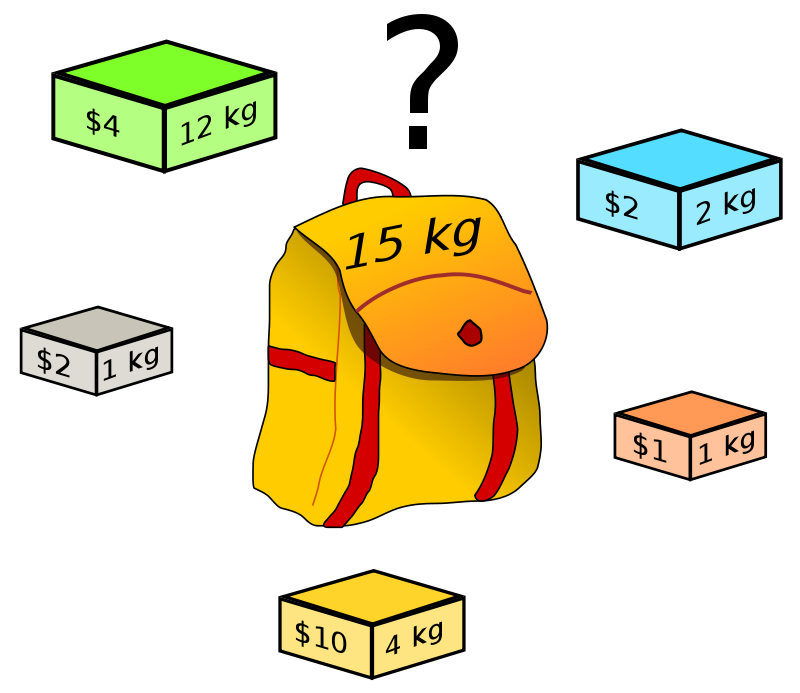
\includegraphics[scale=0.1]{Knapsack.png}
\end{figure}

\end{frame}

\begin{frame}
\frametitle{Sumário}
\tableofcontents
\end{frame}

% CARACTERIZAÇÃO DO PROBLEMA
\section{Caracterização do problema}

\begin{frame}
\frametitle{Definição intuitiva}

    Dado um conjunto de itens, com cada item tendo um peso
    e um custo, qual a escolha de itens tal que a soma de seus pesos é menor
    que a capacidade de uma mochila a soma de seus custos é a maior possível?

\end{frame}

\begin{frame}
\frametitle{Definição matemática: problema de otimização}

    Dados uma mochila com capacidade máxima $W$, um conjunto de $n$ itens $x_{1}, x_{2}, ..., x_{n}$,
    cada um com um peso $w_{i}$ e um valor $v_{i}$:\\

    \begin{equation*}
        \text{maximizar} \sum_{i=1}^{n} v_{i} x_{i}
    \end{equation*}

    \begin{equation*}
        \mbox{sujeito a } \sum_{i=1}^{n} w_{i} x_{i} \leq W \mbox{ e } x_{i} \in \{0,1\}
    \end{equation*}

    Neste caso, $x_{i}$ representa o número de instâncias do item $i$ dentro da mochila.

\end{frame}

\begin{frame}
    \frametitle{Definição matemática: problema de decisão}

    Dados uma mochila com capacidade máxima $W$, um valor mínimo $V$, um conjunto de $n$ itens $x_{1}, x_{2}, ..., x_{n}$,
    cada um com um peso $w_{i}$ e um valor $v_{i}$:\\

    \begin{equation*}
        \text{maximizar} \sum_{i=1}^{n} v_{i} x_{i} \text{ t.q.}
    \end{equation*}

    \begin{equation*}
        \begin{split}
            &\quad \sum_{i=1}^{n} w_{i} x_{i} \leq W \mbox{ e } x_{i} \in \{0,1\} \\
            &\quad \sum_{i=1}^{n} v_{i} x_{i} \geq V \mbox{ e } x_{i} \in \{0,1\} \text{ ?}
        \end{split}
    \end{equation*}

    O problema de decisão se torna: "Existe um seleção de $x_{i}$ que satisfaça essa definição?"

\end{frame}

\begin{frame}
\frametitle{Aplicações}

Aplicações e blabalblabla

\end{frame}

%%%%%%%%%%%%%%%%%%%%%%%%%%%%%%%%%%%%%%%%%%%%%%%%%%%%%%

% PROVA QUE PERTENCE A NP
\section{Problema da mochila binária $\in$ NP}

\subsection{Algoritmo de verificação}
\begin{frame}
    \frametitle{Algoritmo de verificação}
    Para provar que PM\footnotemark $\in$ NP, precisamos mostrar que existe um algoritmo
    capaz de verificar se um certificado do PM é correto em tempo polinomial.

    \footnotetext[1]{PM = Problema da mochila binária}
\end{frame}


\begin{frame}[fragile]
    \frametitle{Algoritmo em pseudocódigo}

    P: conjunto de pesos $p_{i}$ \\
    V: conjunto de valores $v_{i}$ \\
    VMIN: valor minímo para o problema de decisão \\
    W: carga máxima da mochila \\
    n: tamanho do problema
    CERTIFICADO: seleção $x_{1},...,x_{n}\ t.q.\ x \in \{0,1\}$ \\

    \begin{block}{Pré-algoritmo}
    \begin{semiverbatim}
    VerificaPM(P, V, VMIN, W, n, CERTIFICADO)
        ...
        returns SIM or NÃO
    \end{semiverbatim}
    \end{block}

\end{frame}

\begin{frame}[fragile]
    \begin{block}{Algoritmo completo}
        \begin{semiverbatim}
        1. VerificaPM(P, V, VMIN, W, n, CERTIFICADO)
        2.    PesoTotal = 0
        3.    ValorTotal = 0
        4.    for i in 1:n
        5.        PesoTotal += CERTIFICADO[i] * P[i]
        6.        ValorTotal += CERTIFICADO[i] * V[i]
        7.    endfor
        8.    if PesoTotal <= W && ValorTotal > VMIN
        9.        return True
        10.    else
        11.       return false
        \end{semiverbatim}
    \end{block}

\end{frame}

\subsection{Análise de complexidade}
\begin{frame}
    \frametitle{Análise de complexidade}

    \begin{itemize}
        \item As atribuições das linhas 2 e 3 tem complexidade $\mathcal{O}(1)$.

        \item O laço $for$ executa $n$ vezes, e a complexidade das atribuições e multiplicações são constantes.
            A complexidade total do laço é $\mathcal{O}(n)$

        \item A complexidade total do algoritmo é, portanto, $\mathcal{O}(n)$.
        \item O problema da mochila (como problema de decisão) pode, então, ser verificado em tempo polinomial.
              Com isso concluímos que pertence ao conjunto $NP$.
    \end{itemize}

\end{frame}


% PROVA QUE PERTENCE A NP-DIFICIL
\section{Problema da mochila binária $\in$ NP-difícil}

\subsection{Problema NP-difícil usado}
\begin{frame}
    \frametitle{Soma de subconjuntos}
    \begin{itemize}
        \item
            Para demonstrar que PM $\in$ NP-difícil, utilizaremos uma redução do problema
            da soma de subconjuntos para o problema da mochila.
        \item
            Note que estamos utilizando problemas de decisão, mas se demonstrarmos que
            eles pertencem a NP-difícil, é evidente que o problema de otimização associado
            também será NP-difícil (o problema de decisão é mais "fácil").
    \end{itemize}

\end{frame}

\subsection{Redução inst A para inst B}
\begin{frame}
\frametitle{Redução inst A para inst B}
\end{frame}

\subsection{Algoritmo de redução}
\begin{frame}
\frametitle{Algoritmo de redução}
\end{frame}

\subsection{Análise da complexidade}
\begin{frame}
\frametitle{Análise da complexidade}
\end{frame}

\section{Referências}
\begin{frame}
\frametitle{Referências}
\end{frame}

\end{document}

